\chapter{ابزار هدف}
خصیصه‌های مطرح در مدل کیفیتی انتخاب شده، به طور خاص بیان‌گر نحوه اندازه‌گیری نیستند و می‌بایست به منظور رسیدن به یک ابزار درست، در ابتدا مدل‌ کیفیتی انتخاب شده را کمی شفاف‌تر کنیم تا نیازمندی‌ها به صورت دقیق‌تر مشخص شوند. به همین منظور می‌بایست تمامی یازده خصیصه کیفیتی مرتبط با استفاده‌پذیری را به تفصیل شرح داده و روش‌های اتخاذی خود را برای اندازه‌گیری هرکدام مطرح کنیم. از آن‌جا که هدف این پروژه تولید یک نرم‌افزار است، می‌بایست در قدم بعدی به بیان نمودارهای مرتبط بپردازیم و پس از پیاده‌سازی آزمایش‌های لازم را انجام داده و نتایج را ذکر کنیم. در طول این فصل به موارد ذکر شده پرداخته‌ایم که به ترتیب مورد بحث واقع شده‌اند.
\section{نیازمندی‌ها}
ابزار مورد نظر می‌بایست قابلیت اندازه‌گیری استفاده‌پذیری در ذیل مدل کیفیتی مطرح شده در فصل پیشین (مدل تولیس
\cite{albert_measuring_2013})
را داشته باشد. بنابراین توجه به خصیصه‌های کیفیتی مطرح شده در این مدل، اولویت شماره اول است. بررسی مدل‌های کیفیتی مختلف (رجوع شود به جدول
\ref{tab:models})
بیانگر این است که در تبیین مدل‌های کیفیتی به دلیل کل‌نگر بودن و پرهیز از انحصاری شدن، می‌بایست تا حد امکان از بیان جزییات خصیصه‌ها خودداری کرد؛ اما در ساخت ابزارهای آزمون و سنجش کیفیت، بدون داشتن جزییات کافی از نحوه اندازه‌گیری، نخواهیم توانست که به سرمنزل مقصود برسیم. بنابراین می‌توان گفت که مهم‌ترین رسالت این پروژه، پر کردن خلا بین نیازمندی‌های نرم‌افزاری و مدل کیفیتی اتخاذ شده است.
\subsection{تجمیع نتایج پیشین و جمع‌بندی}
\begin{table}[H]
	\caption[
	تجمیع نتایج بررسی بهترین روش‌ها و ابزارها
	]{
		تجمیع نتایج بررسی بهترین روش‌ها و ابزارها؛ مطابق این تجمیع، مشاهده می‌شود که در ابزارها و روش‌ها و تکنیک‌های مطالعه استفاده‌پذیری، هشت الگوی تکراری، به منظور انجام ده سناریوی مهم در مطالعه استفاده‌پذیری استفاده شده‌اند.
	}
	\label{tab:tools_aggregated}
	\centering
	\begin{tabular}{|c|c|}
		\hline
		روش سنجش و اندازه‌گیری & دفعات تکرار الگو \\ \hline
		استفاده از حسگر ردیاب چشم & 4 \\ \hline
		بررسی فنی کد صفحات & 9 \\ \hline
		آزمون‌های مرتبط با حافظه کوتاه‌مدت & 18 \\ \hline
		آزمون پیمایشی & 24 \\ \hline
		پرسش سوالات مربوط به طرح‌های مفهومی & 30 \\ \hline
		آزمون ترجیح & 46 \\ \hline
		ذخیره‌سازی کلیک‌های کاربران و پروفایل‌سازی & 56 \\ \hline
		پرسشنامه متنی و تصویری & 59 \\ \hline
	\end{tabular}
\end{table}
با توجه به جدول
\ref{tab:scenario_measurement}
و همچنین نتایج ذکر شده در انتهای فصل پیشین، می‌توان به منظور درک اهمیت هرکدام از الگوها، مطالعه دیگری انجام داد؛ بد نیست به تجمیع داده‌های موجود در این جدول بیندیشیم. در این صورت به نتیجه بسیار جالب ذکر شده در جدول
\ref{tab:tools_aggregated}
خواهیم رسید که شکل
\ref{fig:tools_aggregation}
نیز بیانگر چهره دیگری از این جدول می‌باشد؛ بر اساس اطلاعات موجود در این شکل، ملاحظه می‌شود که دو الگوی بررسی فنی کد و استفاده از ردیاب، در تعداد کمی از مطالعات مورد استفاده قرار گرفته‌اند. در عمل، این دو الگو به خاطر بررسی مواردی خاص در نظر گرفته شده‌اند که در این موارد به منظور رسیدن به نتیجه‌ای مطلوب، می‌بایست از این‌چنین جزئیاتی نیز اطلاع داشته باشیم. اما نباید از این نکته غافل شد که این دو الگو نیازمند صرف وقت و هزینه بسیار زیادی می‌باشند؛ بدیهی است که برای ثبت داده‌های مربوط به نقطه تمرکز چشم کاربر، نیازمند شرایط، تجهیزات و فضای آزمایشگاهی خاص و گران قیمت خواهیم بود. همچنین به منظور بررسی دقیق و موشکافانه کد تولید شده نهایی، می‌بایست زمان زیادی را در ابتدا برای تولید ابزار طی کنیم که مطلوب ما نیست و می‌توان از سرویس‌هایی آماده و رایگانی همچون
\lr{Google Lighthouse}
استفاده کرد.
\begin{figure}[H]
	\centering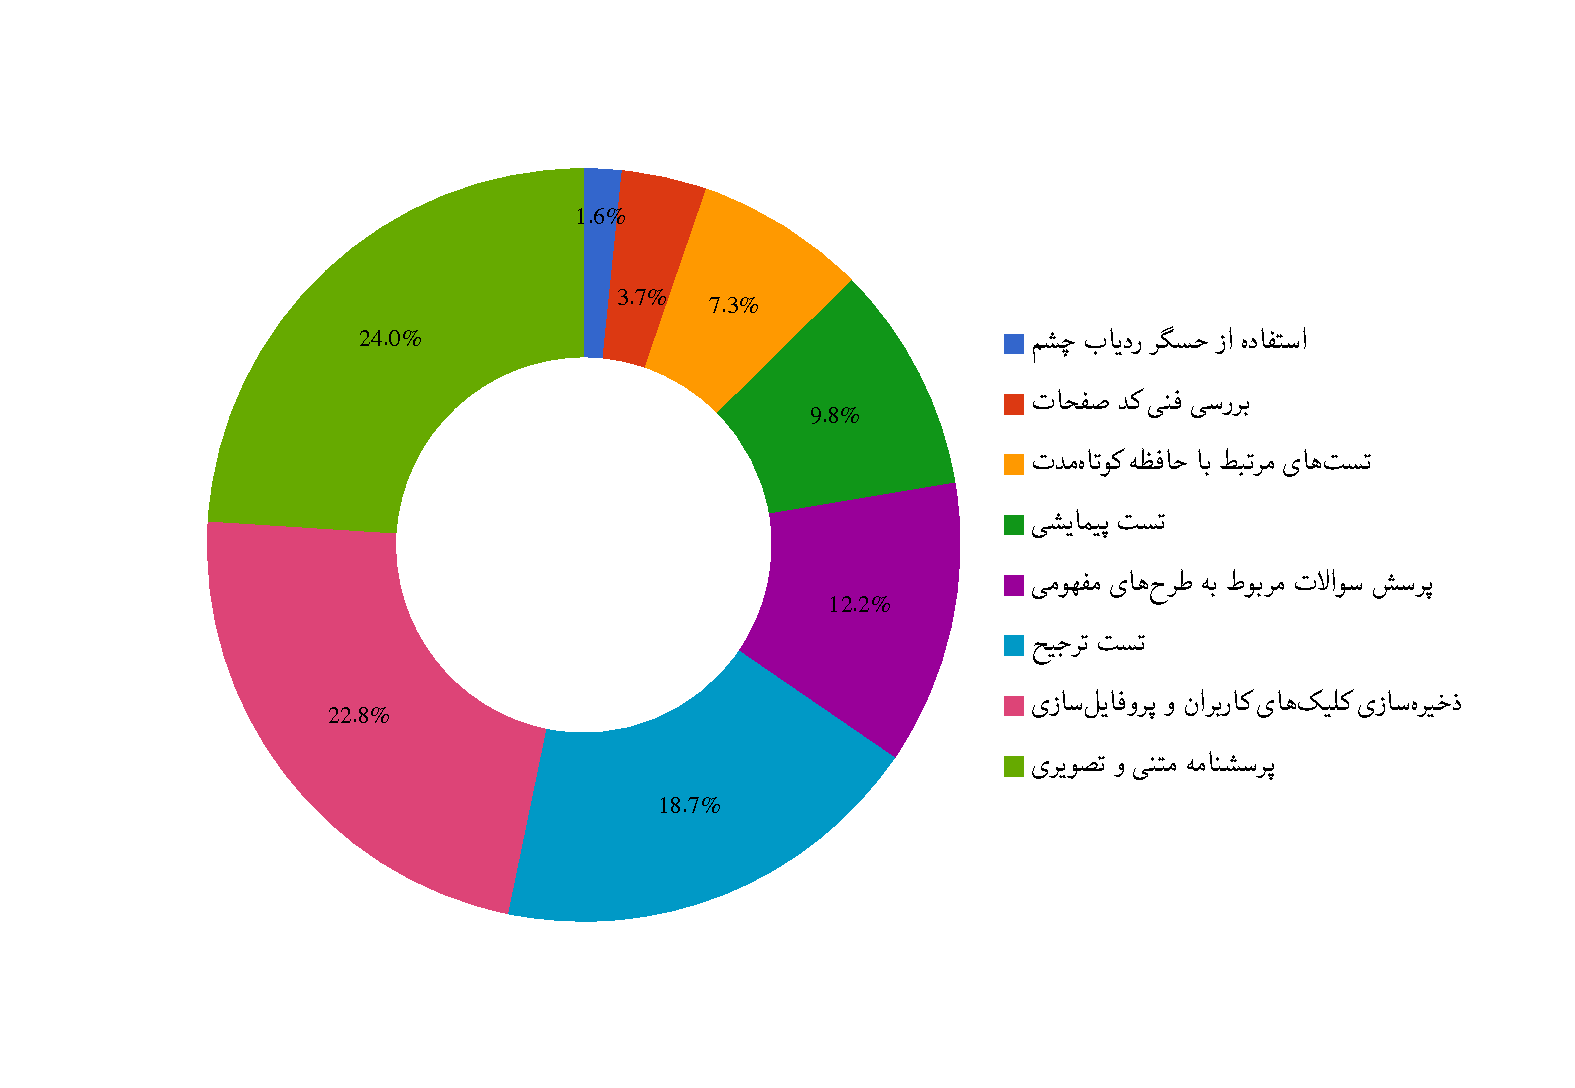
\includegraphics[width=\linewidth]{Resources/percentage.PNG}
	\caption[درصد فراوانی تکرار هر الگو در ابزارهای مورد بررسی]
	{درصد فراوانی تکرار هر الگو در ابزارهای مورد بررسی؛ مشاهده می‌شود که الگوهای ردیابی چشم و همچنین بررسی فنی کد، به دفعات کمتری مورد استفاده قرار گرفته‌اند چرا که کاربر بسیار محدود و جزئی‌ای در مطالعه استفاده‌پذیری دارند. در مقابل اما پرسشنامه‌ها و روش‌های پروفایل‌سازی بیشتر مطرح بوده‌اند.
	}
	\label{fig:tools_aggregation}
\end{figure}
\subsection{تحلیل و پایش}
حال به منظور مرور خصیصه‌های استفاده‌پذیری  و همچنین سناریوهای مطالعه استفاده‌پذیری و نیز اختصاص دادن یک شماره به هرکدام، در ادامه مجددا آن‌ها را یادآوری می‌کنیم؛ مطابق جدول
\ref{tab:10usability}،
سناریو‌های مطالعه استفاده‌پذیری و خصیصه‌های مورد توجه در هر کدام عبارتند از:
\begin{enumerate}
	\item
	انجام یک تراکنش: در این سناریو، خصیصه‌های «موفقیت آمیز بودن وظیفه»، «بهره‌وری کاربر»، «خصیصه‌های موردی»، «خصیصه‌های خود اعلامی» و همچنین «خصیصه‌های وبسایت بلادرنگ» می‌توانند مورد اندازه‌گیری و سنجش قرار می‌گیرند.
	\item
	مقایسه محصولات: با انجام این سناریو، می‌توان خصیصه‌های «موفقیت‌آمیز بودن وظیفه»، «بهره‌وری کاربر»، «خصیصه‌های خوداعلامی» و همچنین «خصیصه‌های ترکیبی و مقایسه‌ای» را مورد بررسی، سنجش و اندازه‌گیری قرار داد.
	\item
	ارزیابی استفاده مکرر از محصول: که در صورت انجام، «موفقیت‌آمیز بودن وظیفه»، «زمان انجام وظیفه»، «بهره‌وری»، «یادگیری‌پذیری» و نیز «خصیصه‌های خود اعلامی» را می‌توان مورد سنجش قرار داد.
	\item
	ارزیابی پیمایش و معماری اطلاعات سامانه: با اجرای این سناریو می‌توان «موفقیت‌آمیز بودن وظیفه»، «خطاها»، «بهره‌وری کاربر» و همچنین «الگوهای مرتب‌سازی» را مورد سنجش و ارزیابی قرار داد.
	\item
	افزایش آگاهی: با انجام مطالعه استفاده‌پذیری به منظور رسیدن به این هدف، می‌توان «خصیصه‌های خوداعلامی»، «خصیصه‌های فیزیولوژیکی و رفتاری» و همچنین «خصیصه‌های وبسایت‌ بلادرنگ» را مورد بحث و بررسی قرار داد.
	\item
	کشف مشکل: با در نظر قرار دادن این سناریو در انجام مطالعات استفاده‌پذیری، می‌توان «خصیصه‌های موردی» و «خصیصه‌های خوداعلامی» را مورد سنجش و ارزیابی قرار داد.
	\item 
	حداکثرسازی استفاده‌پذیری یک محصول حیاتی: هنگامی که این هدف مدنظر باشد، می‌توان «موفقیت‌آمیز بودن وظیفه»، «خطاها» و «بهره‌وری کاربر» را مورد توجه، سنجش و ارزیابی قرار داد.
	\item 
	ایجاد تجربه کاربری مثبت:
	در مطالعه استفاده‌پذیری به منظور ایجاد تجربه کاربری مثبت، «خصیصه‌های خوداعلامی» و همچنین «خصیصه‌های فیزیولوژیکی و رفتاری» که جزئی از ویژگی‌های کاربر نیز هستند، می‌توانند مورد توجه، ارزیابی و سنجش قرار بگیرند.
	\item 
	ارزیابی تاثیرات تغییرهای جزئی و نامحسوس: اگر مطالعه‌ای با این هدف انجام بگیرد، می‌تواند خصیصه‌ای همچون «خصیصه‌های وبسایت بلادرنگ» را با جزئیات زیادی مورد توجه خود واقع کند و به سنجش آن‌ها بپردازد.
	\item
	مقایسه طراحی‌های مختلف: که بیشتر به منظور بیشینه کردن راحتی کاربران هستند، می‌توانند برای سنجش و ارزیابی «موفقیت‌آمیز بودن وظیفه»‌، «زمان انجام وظیفه»، «خصیصه‌های موردی»، «خصیصه‌های خوداعلامی» و همچنین «خصیصه‌های ترکیبی و مقایسه‌ای» به کار گرفته شوند.
\end{enumerate}
\begin{table}[H]
	\caption[
	نیازمندی‌های کشف‌شده برای ابزار هدف
	]{
		نیازمندی‌های کشف‌شده برای ابزار هدف؛ این نیازمندی‌ها از روی الگوهای مطالعه و سنجش استفاده‌پذیری به دست آمده‌اند و طبق اطلاعات این جدول، به نظر می‌رسد که در صورت استفاده از این الگو، می‌توان بعد کاملی از مدل کیفیتی را، در مورد مطالعه استفاده‌پذیری، به کار برد. دقت شود که اعداد مربوط به سناریوهای مطالعه استفاده‌پذیری، اعداد ذکر شده در متن هستند.
	}
	\label{tab:requirements}
	\centering
	\begin{tabular}{|C{3cm}|C{3cm}|C{8cm}|}
		\hline
		الگو & سناریو(ها)ی قابل انجام & نیازمندی ابزار \\ \hline
		پرسشنامه متنی و تصویری & ۱، ۲، ۴، ۶، ۸، ۹، ۱۰ & دارا بودن امکان آپلود تصاویر و متون متعدد در قالب یک پرسشنامه و همچنین جمع‌آوری پاسخ کاربران \\ \hline
		ذخیره‌سازی کلیک‌های کاربران و پروفایل‌سازی & ۱، ۳، ۴، ۶، ۷، ۸ & استفاده از زبان تحت وبی که به رخدادهای مرورگر پاسخ دهد \\ \hline
		آزمون ترجیح & ۲، ۵، ۷، ۸، ۹، ۱۰ & دارا بودن امکان آپلود تصاویر متعدد و نمایش آن‌ها در کنار هم و جمع‌آوری پاسخ کاربران \\ \hline
		پرسش سوالات مربوط به طرح‌های مفهومی & ۵، ۶، ۸، ۱۰ & دارا بودن امکان آپلود تصاویر و متون متعدد در قالب یک پرسشنامه و همچنین جمع‌آوری پاسخ کاربران \\ \hline
		آزمون پیمایشی & ۱، ۳، ۴ & دارا بودن امکان نمایش چندین عکس به طور متوالی و ذخیره پاسخ کاربر و زمان سپری شده توسط وی روی هرکدام \\ \hline
		آزمون‌های مرتبط با حافظه کوتاه مدت & ۲، ۳، ۹ & استفاده از زبانی که به رخدادهای مرورگر پاسخ دهد و همچنین قابلیت نمایش زمان‌دار موارد به کاربر \\ \hline
	\end{tabular}
\end{table}
با استفاده از اطلاعات ذکر شده و با توجه به تعریف‌هایی که از خصیصه‌های کیفیتی در فصل سوم مطرح شد، با نگاهی بر ابزارهای مطرح و روش‌های اندازه‌گیری آن‌ها و توجه به این نکته که این روش‌ها و ابزارها، در زمان نگارش این اثر، جزو بهترین روش‌ها\LTRfootnote{
	Best Practice
}
و ابزارهای موجود می‌باشند، می‌توان به طور خلاصه استراتژی مطرح برای اندازه‌گیری هر کدام از خصیصه‌ها را در قالب جدول
\ref{tab:requirements}
مطرح کرد؛ توجه به این نکته حائز اهمیت است که از دو الگوی هزینه‌بر ذکر شده صرف نظر شده است و نهایتا در ابزار هدف، به منظور اندازه‌گیری و سنجش خصیصه‌های کیفیتی مطرح شده در مدل تولیس، از ۶ الگوی مطرح شده در جدول
\ref{tab:requirements}،
استفاده می‌شود.\\
با توجه به پوشا بودن این نیازمندی‌ها\RTLfootnote{
	به این معنا که در صورت پیاده‌سازی شدن این نیازمندی‌ها، یک بعد از مدل کیفیتی که در مطالعات برخط می‌توان به آن‌ها پرداخت، به تمامی قابل حصول است و در واقع در مطالعه استفاده‌پذیری با این ابزار، می‌توان مطمئن شد که تمامی خصیصه‌های کیفیتی را می‌توان مورد سنجش و اندازه‌گیری قرار داد؛ چرا که طبق جدول‌های 
		\ref{tab:tools_category}
		و 
		\ref{tab:requirements}
		در صورت قادر بودن به انجام سناریوهای ذکر شده، می‌توان تمام خصیصه‌های مطرح در مدل کیفیتی را مورد سنجش و ارزیابی قرار داد.
}، می‌بایست به جنبه دیگر نیازمندی‌ها -نباید غافل شد که ما در پی ساخت ابزاری به منظور مطالعه استفاده‌پذیری به صورت برخط و با استفاده از جمع‌سپاری هستیم- پرداخت. با توجه به اینکه این ابزار در دسترس افراد زیادی خواهد بود، می‌بایست مدیریت حساب، احراز هویت، و حفظ حریم خصوصی افراد، به عنوان یک نیازمندی مهم مدنظر باشد.\\
همچنین از جدول
\ref{tab:requirements}
برمی‌آید که یک نیازمندی پنهان نیز کشف شده است و آن چیزی نیست جز، الزام پاسخگو بودن زبان مورد استفاده به رخدادهای مرورگر. باید در نظر داشت که ابزارهای ذکر شده در جدول
\ref{tab:tools}
از زبان‌های
«Java»
گرفته تا زبان‌های
«PHP»
و حتی چارچوب‌های برنامه‌نویسی‌ای\LTRfootnote{Framework}
همچون
«.Net»
مایکروسافت تا چارچوب
«Django»
را استفاده کرده‌اند و نمی‌توان قضاوت خاصی از روی تاریخچه استفاده این ابزارها از زبان یا چارچوب خاصی کرد. اما با مشاهده راستای\LTRfootnote{Trend}
تکنولوژی سامانه‌های تحت وب، می‌توان گفت که زبان
«Javascript»
و به طور خاص چارچوب
«Nuxt.js»
می‌تواند برای پروژه جاری بسیار مناسب باشد. جمله پیشین بدون منبع آکادمیک است؛ ولی در جمع توسعه‌دهندگان اهل فن، پذیرفته و بدیهی به نظر می‌رسد و می‌توان آن را یک
«Best-Practice»
در نظر گرفت
\cite{noauthor_curated_2018, sozo_10_2018, noauthor_creating_nodate}؛
از طرفی  باید در نظر داشت که سامانه‌های کاربردی تحت وب تک صفحه\LTRfootnote{Single Page Applications (SPAs) on Web}
به آسانی توسط این چارچوب زبان
«Javascript»
قابل توسعه و پیاده‌سازی هستند که گزینه ایده‌آلی برای این پروژه می‌باشند
\cite{ardalis_choose_nodate, neoteric_single-page_2016}.\\
به عنوان طراح و مجری یک ابزار با هدف افزایش استفاده‌پذیری و با در نظر گرفتن این حقیقت که استفاده‌پذیری ارتباط تنگاتنگی با کاربر نهایی دارد، می‌بایست همواره مخاطب خود را شناسایی کنیم؛ چرا که از جمله‌ اساسی‌ترین حقیقت‌ها در مهندسی نرم‌افزار، تطابق حداکثری نیازمندی‌ها با محصول نهایی است
\cite{sommerville_software_2016}.
بنابراین مخاطب یک سامانه، عامل اصلی تعیین‌کننده موفقیت آن سامانه در ارضای نیازهای وی است که استفاده‌پذیری نیز از این اصل جدا نیست. بنابراین لازم است در مطالعه استفاده‌پذیری سلایق و نظرات کاربران همجوار با محدوده کاربران محصولات خود را در نظر گرفته و از آن‌ها به عنوان فرصتی برای افزایش کیفیت محصولات خود استفاده کنیم.\\
اما شایان ذکر است که استفاده وسیع (در دسترس بودن برای عموم)، از جمله ویژگی‌هایی است که برخی ملاحظات امنیتی از جمله مقابله با هرزنامه‌ها را نیز به همراه دارد. مجددا به عنوان طراح ابزاری که از جمع‌سپاری برای نتیجه‌گیری استفاده می‌کند، همانطور که مطالعات متعددی از جمله
\cite{li_crowdsourced_2016}
نشان می‌دهند، می‌بایست در نظر داشته باشیم که کیفیت خروجی نهایی ممکن است بسیار دستخوش تغییرات نامطلوب گردد و به همین جهت، می‌بایست تدابیری برای کنترل و مدیریت کیفیت فرآیند جمع‌سپاری در نظر داشته باشیم. با در نظر گرفتن فصل پیشین و با بررسی روش‌های موجود، می‌توان استفاده از رویکرد مدل‌سازی کارگران را یک راه‌حل مناسب برای این چالش فعلی دانست. چرا که کیفیت حداقلی را تضمین کرده و هزینه زیادی نیز متحمل نخواهد کرد: تضمین حداقلی کیفیت به خاطر این است که آزمون‌گر می‌تواند پاسخ‌هایی که کیفیت مطلوبی ندارند را از گردونه محاسبات خارج کرده و در تحلیل‌های نهایی، تاثیری از پاسخ‌های بی‌کیفیت نباشد. باید توجه داشت که این روش، مساوی و معادل با روش حذف کارگران بی‌کیفیت نیست. چرا که در اینجا ساده‌ترین حالت فرض شده و هیچ پروفایلی برای کاربران ساخته نمی‌شود. بنابراین بعد دیگری از نیازمندی‌های ابزار را اینجا نیز بررسی کردیم.\\
\subsection{مهندسی نیازمندی‌ها}
توجه به این نکته حائز اهمیت خواهد بود که به منظور تحلیل دقیق و طراحی درست سیستم می‌بایست از در بسیاری از موارد از ذکر جزییات خودداری کرده و سامانه را از منظری بزرگتر و با هدفی دیگر نگاه کرد؛ به عبارتی دیگر می‌بایست با توجه به سطوح تجرید مختلف، مدل‌سازی کرد. یکی از ابزارهای مطرح در مهندسی نرم‌افزار به منظور مدل‌سازی، زبان مدل‌سازی یکپارچه\LTRfootnote{Unified Modeling Language} است. که یک زبان شی‌گرا است. شی‌گرایی، باعث شده که در توسعه مدل‌های فرمال و صوری برای سامانه‌های نرم‌افزاری، به جای تمرکز به دنیای ماشین‌ها، ذهن خود را در دنیای اطرافمان حاضر ببینیم و مدلی بسیار نزدیک‌تر، واقعی‌تر و قابل فهم‌تر بسازیم. سامانه‌ها و ابزارهای مبتنی بر وب نیز بر همین اساس، می‌توانند توسط این زبان مدل‌سازی شده و طراحی گردند. به همین منظور، با توجه به مطالبی که در طول این فصل و فصل‌های پیشین گفته شد و نیازمندی‌هایی که مطرح شدند، در ابتدای کار طراحی، مدل نیازمندی‌های ابزار خود را بازگو می‌کنیم.\\
مطابق شکل
\ref{fig:usecase}،
ملاحظه می‌شود که دو نقش تعریف کننده آزمون و شرکت کننده آزمون در با ابزار در ارتباط خواهند بود. تعریف‌کننده آزمون در واقع همان طراح، شرکت و یا سازمانی است که قصد افزایش استفاده‌پذیری محصول مورد سنجش را دارد و شرکت‌کننده آزمون، در واقع همان کاربر نهایی است که بدون نیاز به احراز هویت، روی سامانه، رابط‌های کاربری مختلفی را مورد سنجش قرار می‌دهد و به سوالاتی که تعریف‌کنندگان آزمون طرح کرده‌اند پاسخ خواهد داد.
\begin{figure}[H]
	\centering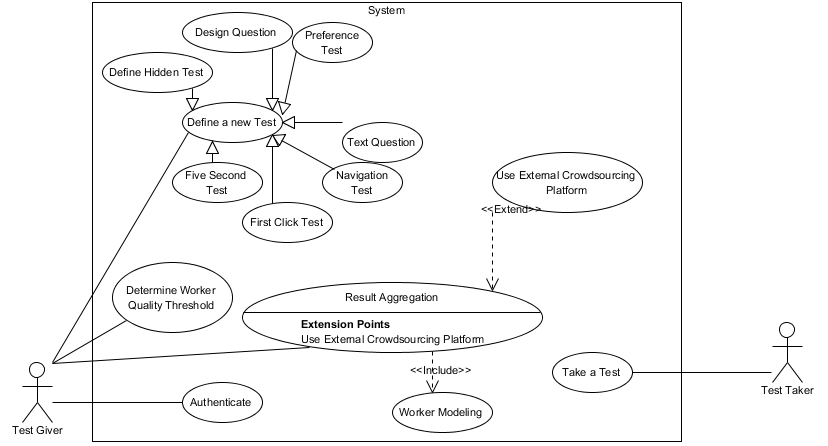
\includegraphics[width=\linewidth]{Resources/UseCaseDiagram.PNG}
	\caption[نمودار مورد کاربرد سامانه هدف]{
		نمودار مورد کاربرد\LTRfootnote{Use Case Diagram}
		ابزار هدف
	}
	\label{fig:usecase}
\end{figure}
\subsubsection{مدل‌سازی جنبه‌های دینامیک سیستم}
با توجه به نمودار مورد کاربرد، می‌توان مواردی از استفاده را مشاهده کرد که جزییات انجام آن‌ها برای خواننده ممکن است کمی گنگ باشد. به همین منظور به سراغ نمودارهای فعالیت\LTRfootnote{Activity Diagram}\RTLfootnote{رعایت نگارش زبان فارسی، البته که در اولویت بوده ولی کماکان برخی لغات و اصطلاحات تخصصی، به خصوص در مهندسی نرم‌افزار، هستند که عبارات ترجمه شده آن‌ها کامل گویا نبوده و یا هنوز به دلیل نو و بدیع بودن، نتوانسته‌اند جایگاه خود را بگیرند. اینجانب تا حد امکان سعی در عدم استفاده از عبارات لاتین و حفظ نگارش زبان فارسی داشته‌ام و به همین جهت همواره در متن فارسی، از معادل فارسی کلمات، که گاهی همراه با پانویس هستند استفاده کرده‌ام؛ امید است که استفاده زیاد از پانویس، خواننده را ملول نکند!}
می‌رویم که در شکل
قابل مشاهده هستند. در مورد نحوه تعریف آزمون جدید، همانطور که مطرح شد، شش الگو مطرح شدند که در ادامه نحوه تعریف هرکدام از الگوها را مورد بررسی قرار داده‌ایم. در شکل
\ref{fig:aggactivity}
نمودار فعالیت مربوط به واکشی نتایج برگزاری یک آزمون قابل مشاهده است؛ مطابق این نمودار، ابتدا درخواست واکشی نتایج از سمت صاحب آزمون به ابزار داده می‌شود؛ ابزار با توجه به آستانه کیفیتی که قبلا توسط صاحب آزمون تعیین شده است، پاسخ‌های دریافت شده از آزمون را، چه از سکوهای خارجی (در اینجا چون فقط با یک سکو از طریق واسط برنامه‌نویسی وصل است، تنها با
«\lr{Figure-Eight}»\RTLfootnote{
	این سکو، درواقع همان سکوی
	«\lr{CrowdFlower}»
	می‌باشد که به تازگی و در سال ۲۰۱۸ تغییر نام داده و به 
	«\lr{Figure-Eight}»
	تبدیل شده است.
})
و چه از پایگاه داده خود ابزار جمع‌آوری می‌کند (تمامی جواب‌ها). در دور اول، ابتدا برای تمام آن‌ها و مطابق آزمون‌های مخفی نهانده شده در هر مورد آزمون\LTRfootnote{Test Case}
$q$
را مورد محاسبه قرار می‌دهد تا کیفیت آن نتیجه به دست آید. پس از مرتب‌سازی نتایج، با توجه به مقداری که صاحب آزمون، به عنوان آستانه کیفیت پاسخ‌ها در نظر گرفته، مواردی که از میزان مشخص شده کمتر بودند در نظر گرفته نمی‌شوند و برای اعلام نتیجه نهایی، تحویل تابع نتیجه‌ده می‌شوند. عملکرد این تابع مطابق با نوع مورد آزمون می‌تواند متفاوت باشد.
\begin{figure}
	\centering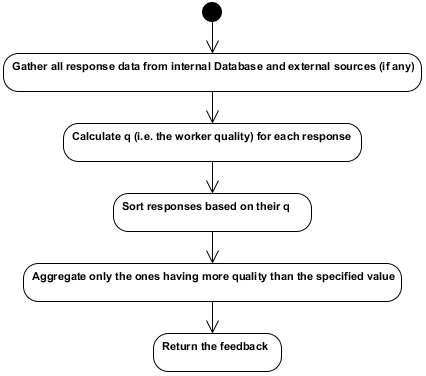
\includegraphics[width=0.7\linewidth]{Resources/AggregationActivityDiagram.PNG}
	\caption{
		نمودار فعالیت مربوط به واکشی نتایج برگزاری آزمون سنجش استفاده‌پذیری
	}
	\label{fig:aggactivity}
\end{figure}
\begin{figure}
	\centering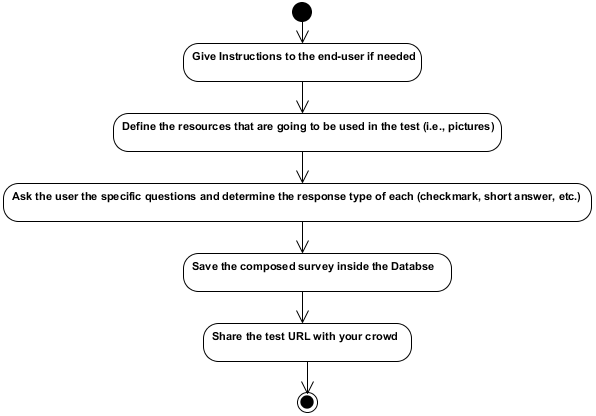
\includegraphics[width=0.7\linewidth]{Resources/DefineActivityDiagram.PNG}
	\caption[نمودار فعالیت مربوط به تعریف آزمون‌های مختلف]{
		نمودار فعالیت مربوط به تعریف آزمون‌های مختلف؛ آزمون‌های مختلف صرفا با تفاوت فرم‌هایی از یکدیگر جدا می‌شوند. ساختار داده‌ای آن‌ها یکسان است.
	}
	\label{fig:defactivity}
\end{figure}
در شکل
\ref{fig:defactivity}
نیز نحوه تعریف یک مورد آزمون جدید قابل مشاهده است. صاحب آزمون پس از انجام تعاریف مورد نظر و دادن اطلاعات مورد نیاز به کاربر، سوالات خود از وی را می‌پرسد و نحوه پرسش سوالات را نیز مشخص می‌کند؛ به این صورت صاحب آزمون می‌تواند آزمونی را تعریف کرده و نیازمندی‌های خود را از کاربران نهایی بپرسد.
\begin{figure}
	\centering
	\subfloat[فرم تعریف یک آزمون]{
		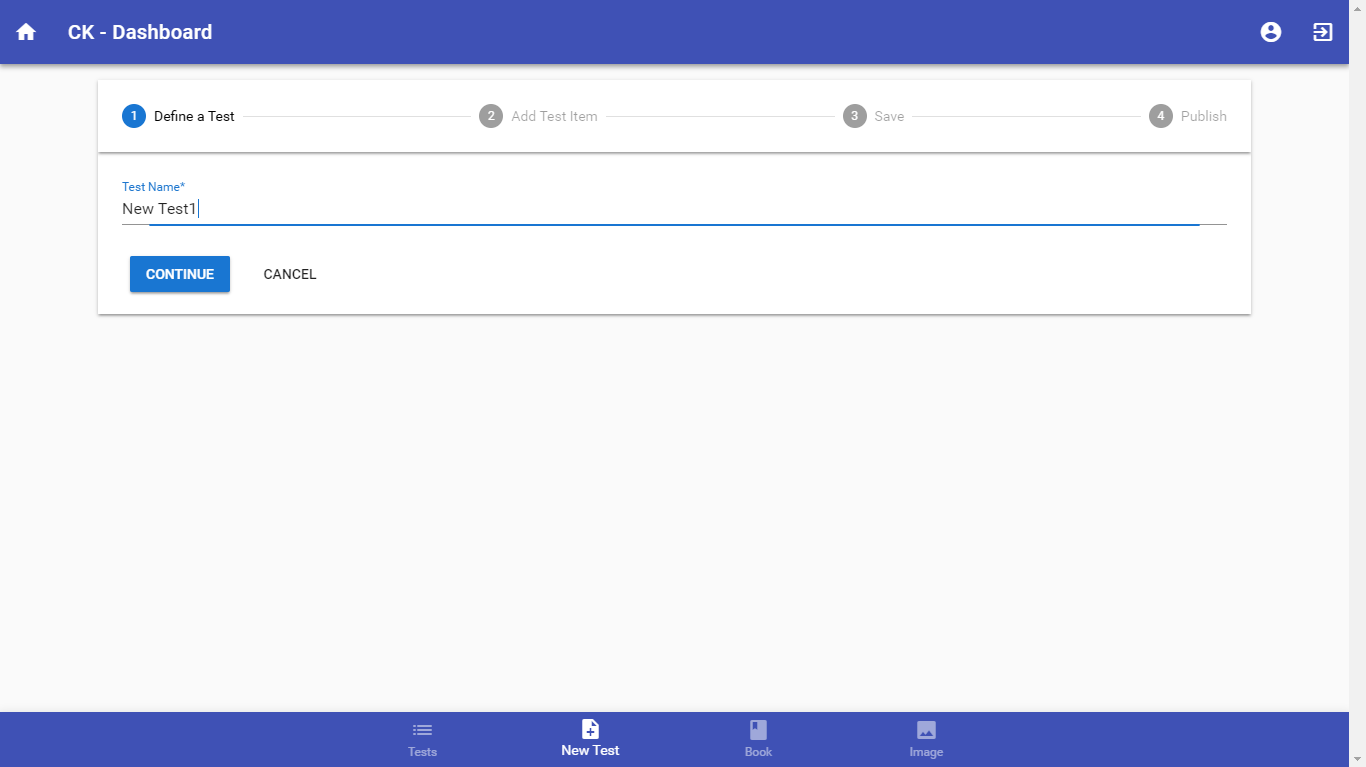
\includegraphics[width=7.5cm]{Resources/screen1.PNG}
	}
	\subfloat[افزودن یک مورد آزمون به آزمون کلی]{
		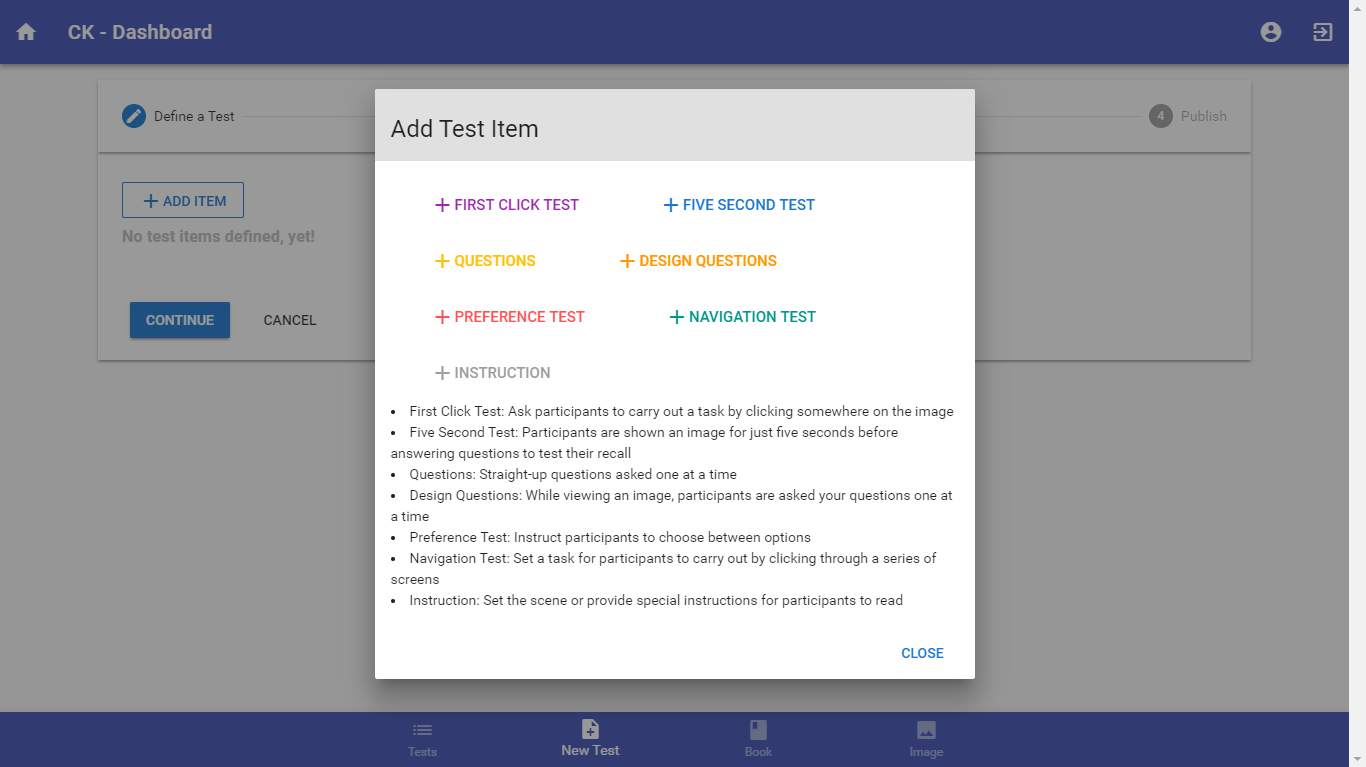
\includegraphics[width=7.5cm]{Resources/screen2.PNG}
	}
	\hspace{0mm}
	\subfloat[فرم ویرایش یک مورد آزمون]{
		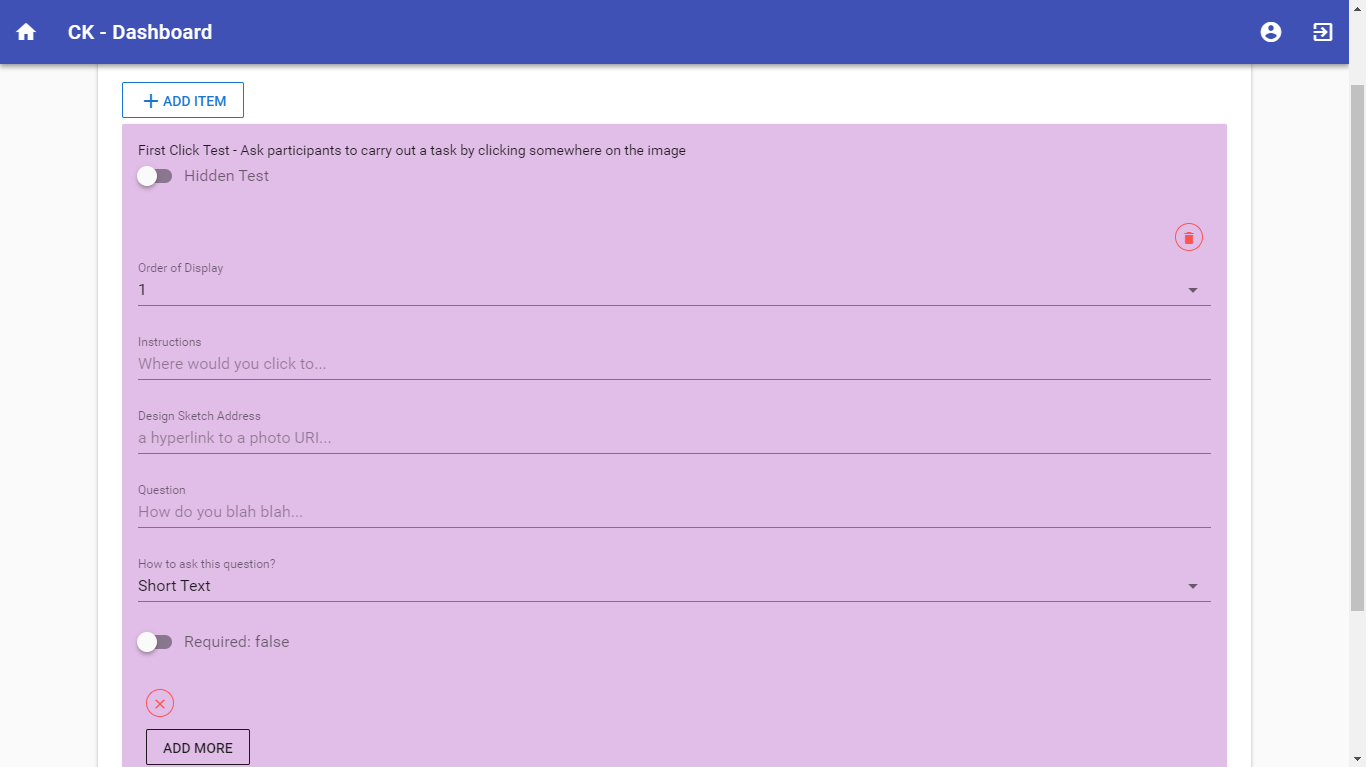
\includegraphics[width=7.5cm]{Resources/screen3.PNG}
	}
	\subfloat[ذخیره آزمون]{
		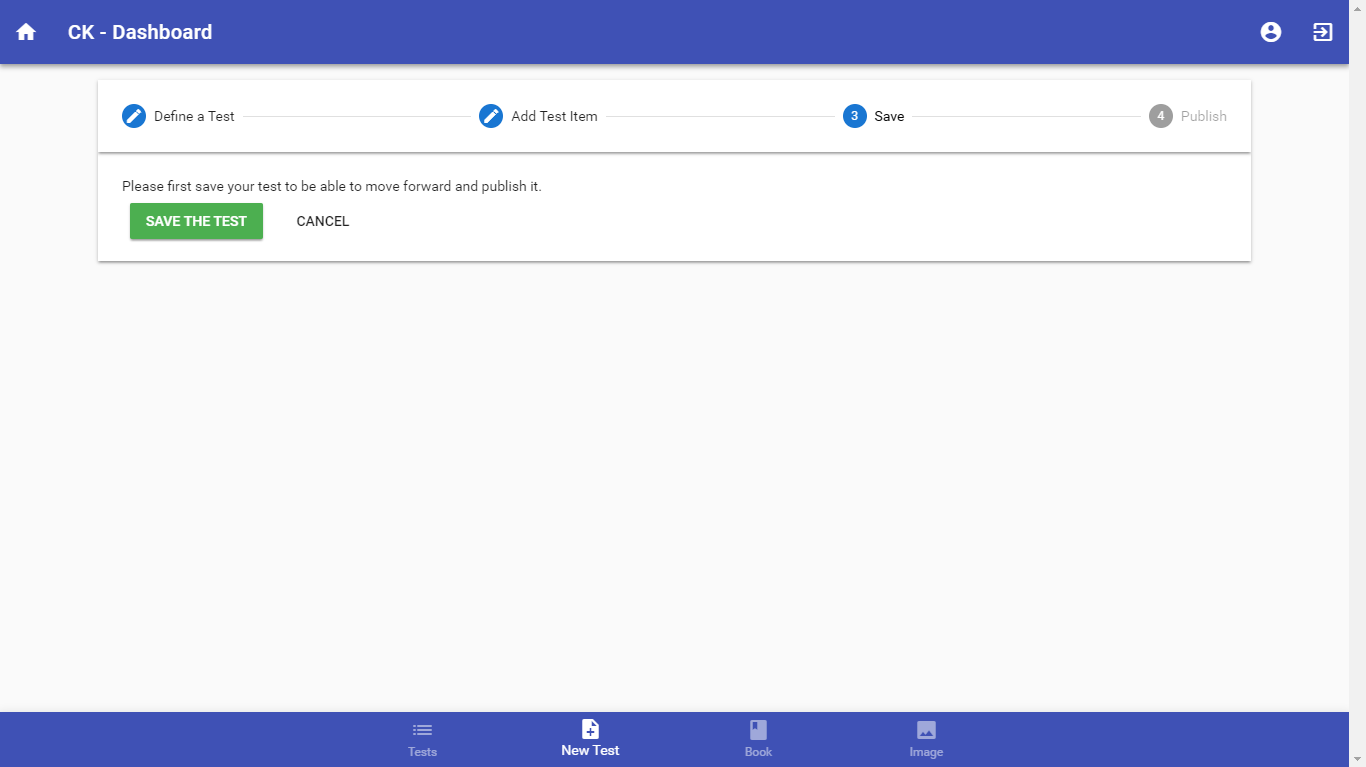
\includegraphics[width=7.5cm]{Resources/screen4.PNG}
	}
	\hspace{0mm}
	\subfloat[ارسال درخواست جمع‌سپاری به سکوی
	\lr{Figure-Eight}
	]{
		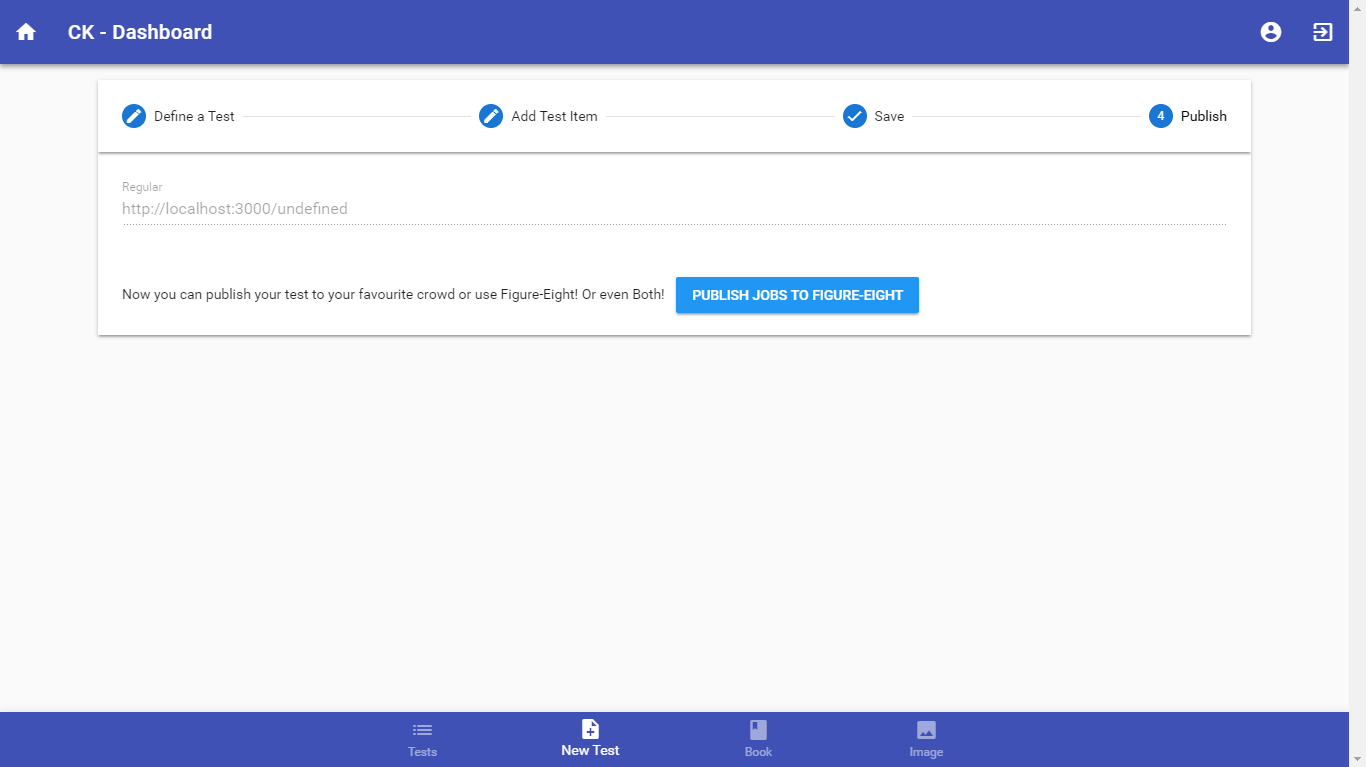
\includegraphics[width=7.5cm]{Resources/screen5.PNG}
	}
	\caption[روند تعریف یک آزمون در ابزار]
	{روند تعریف یک آزمون در ابزار
	}
	\label{fig:pages}
\end{figure}
کاربران پس از ورود به حساب کاربری خود در سامانه، می‌توانند لیست آزمون‌های پیشین خود را مشاهده و در صورت لزوم در آن‌ها تغییری ایجاد کنند، حساب خود را مدیریت کنند و یا به ایجاد آزمون جدید بپردازند. پس از اینکه آزمون جدید ساخته شد و منتشر گردید، کاربر دارای آدرس وب منحصر به فردی خواهد شد که به طور خاص برای آزمون مدنظرش است؛ علاوه بر اینکه کاربر می‌تواند مطابق شکل
\ref{fig:pages}
 با به اشتراک گذاشتن آدرس وب با همگان، آن‌ها را دعوت به شرکت در انجام آزمون از طریق سامانه بکند، می‌تواند از امکان استفاده از سکوی جمع‌سپاری
«\lr{Figure-Eight}»
که با ابزار مورد نظر با واسط برنامه‌نویسی آن سکو ادغام شده است، بهره ببرد.\\


















